\section{Adapting the IIM methods to other discretisation schemes}

This section discusses the adaptations necessary to use the methods mentioned in the previous three sections with more complex discretisation schemes than the FTCS method.

The addition of extra points to the finite difference stencil increases the complexity of the IIM because there are now extra locations where the interface crosses the grid, and thus extra locations that require correction.
Figures \ref{fig:FDGrid}, \ref{fig:BDGrid} and \ref{fig:CNGrid} illustrate this with three spatially second-order discretisations with different time discretisations.

\begin{figure}[h]
    \centering
    \begin{subfigure}[b]{0.3\textwidth}
        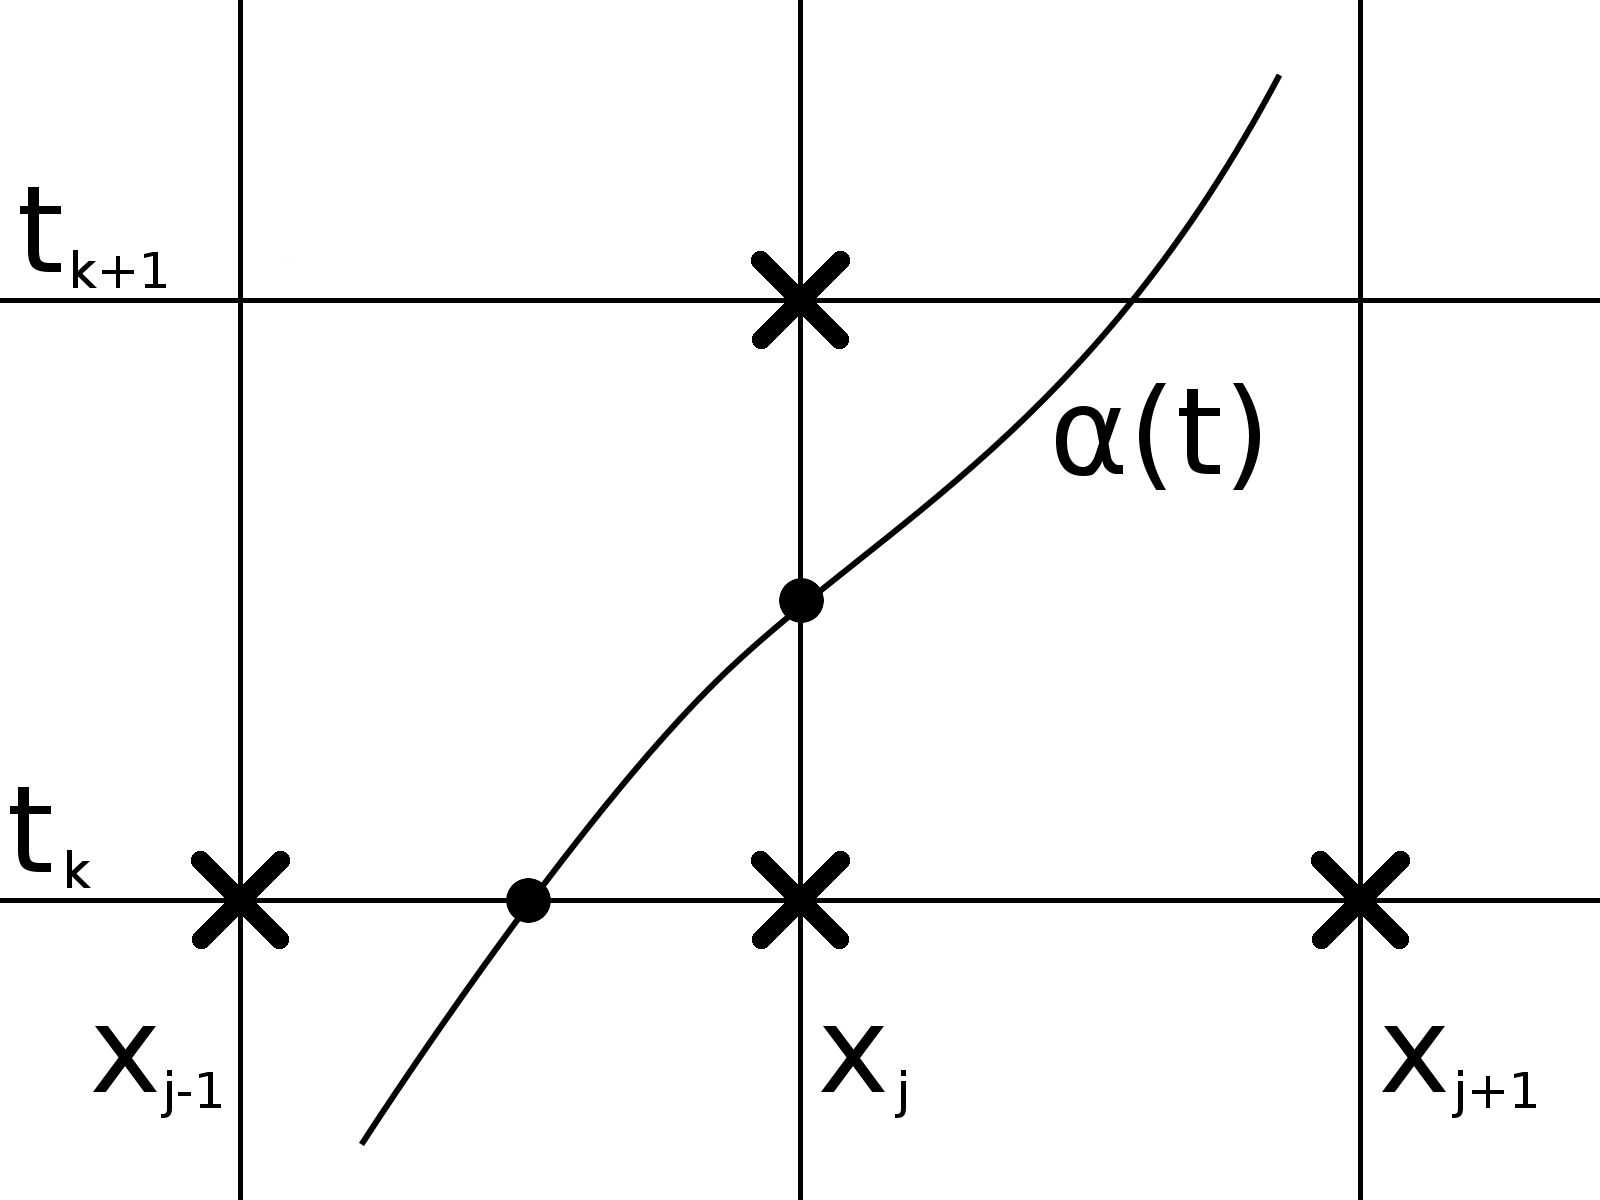
\includegraphics[width=\textwidth]{diagrams/GridFD}
        \caption{Forward-time}
        \label{fig:FDGrid}
    \end{subfigure}
    \begin{subfigure}[b]{0.3\textwidth}
        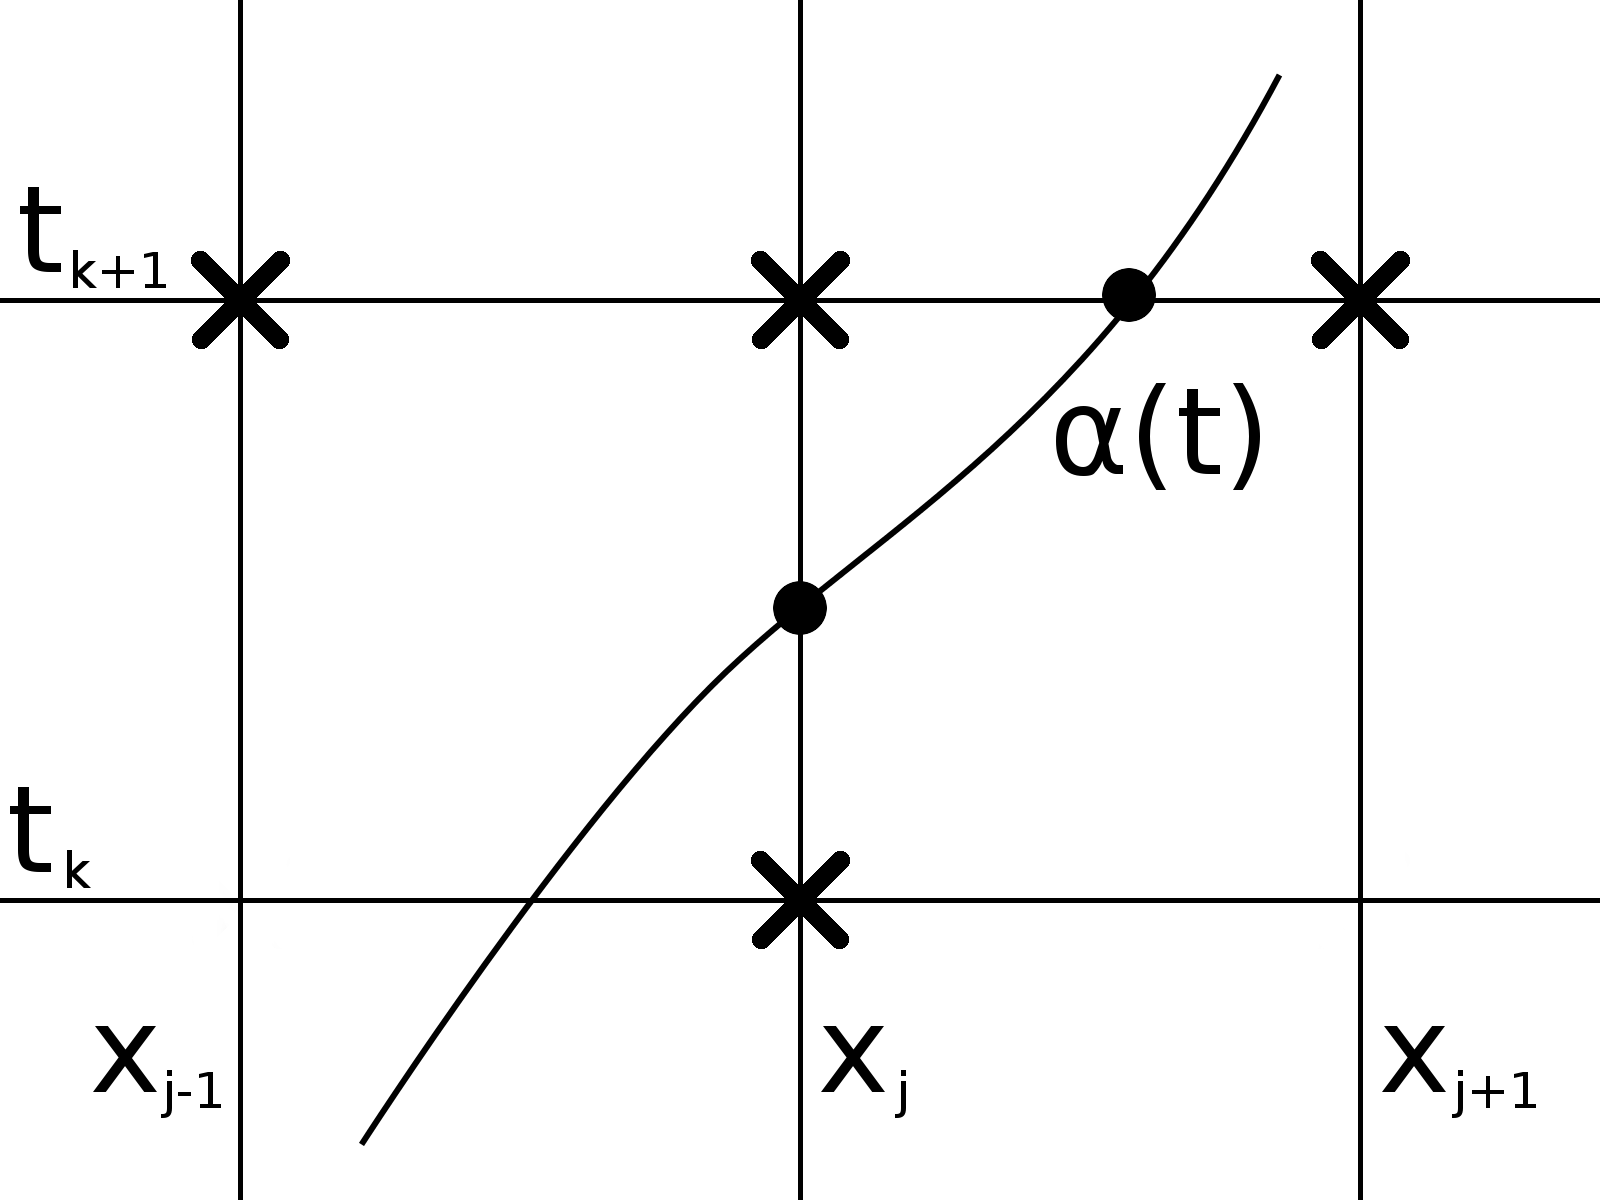
\includegraphics[width=\textwidth]{diagrams/GridBD}
        \caption{Backward-time}
        \label{fig:BDGrid}
    \end{subfigure}
    \begin{subfigure}[b]{0.3\textwidth}
        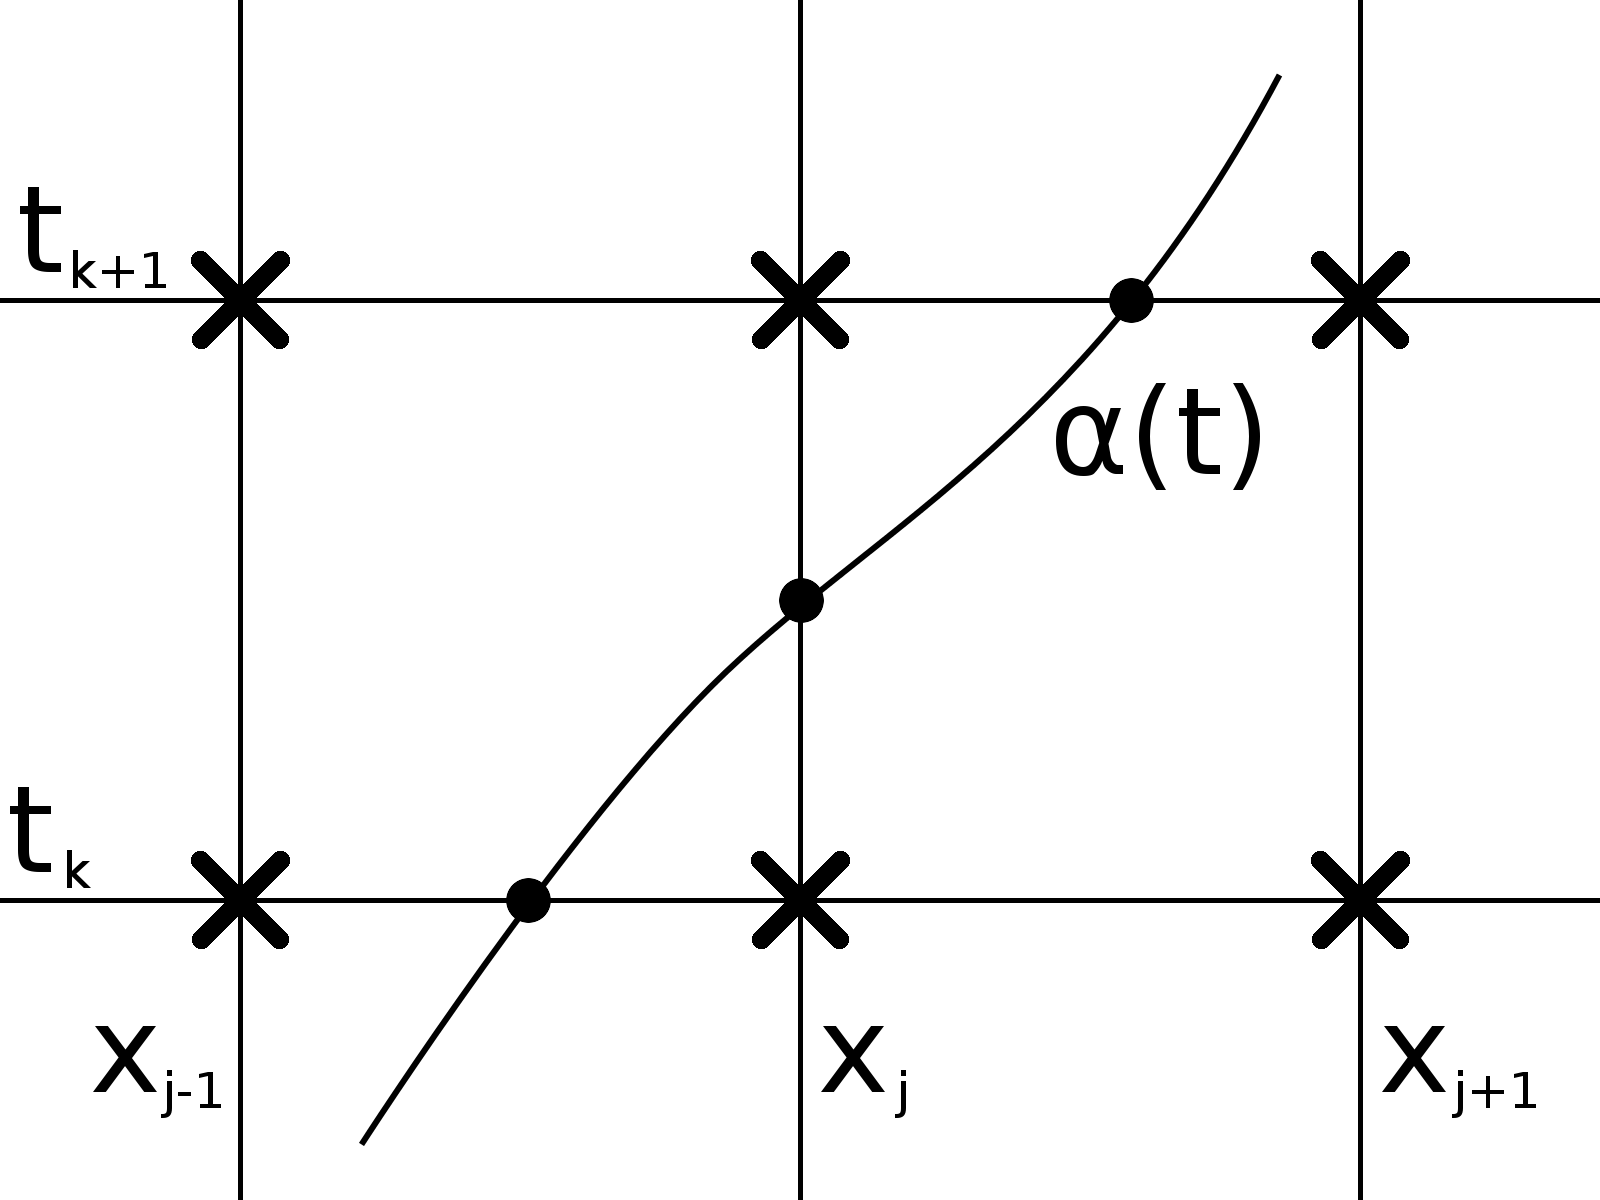
\includegraphics[width=\textwidth]{diagrams/GridCN}
        \caption{Crank-Nicolson}
        \label{fig:CNGrid}
    \end{subfigure}
    \caption{The finite difference stencil for three different spatially second order discretisation schemes.
    The interface $\alpha(t)$ is drawn, and the locations where the interface cuts the finite difference stencil are indicated with black dots.
    These locations will require a time correction if they lie on an $x$ gridline or a space correction if they lie on a $t$ gridline}
    \label{fig:GridCrossing}
\end{figure}

In addition to varying with the discretisation scheme used, the location of these correction points also varies with the sign of $d \alpha / dt$.
Although the examples considered in this project all use monotonic functions for $\alpha(t)$, there may be situations where the movement of the interface displays some nonmonotonic behavior.
It is also necessary to consider what effect this would have on problems in two spatial dimensions, where the grid crossings can now occur in two dimensions, as well as in the time dimension if the interface is moving (see figure \ref{2DGrid}).

\begin{figure}[h]
    \centering
    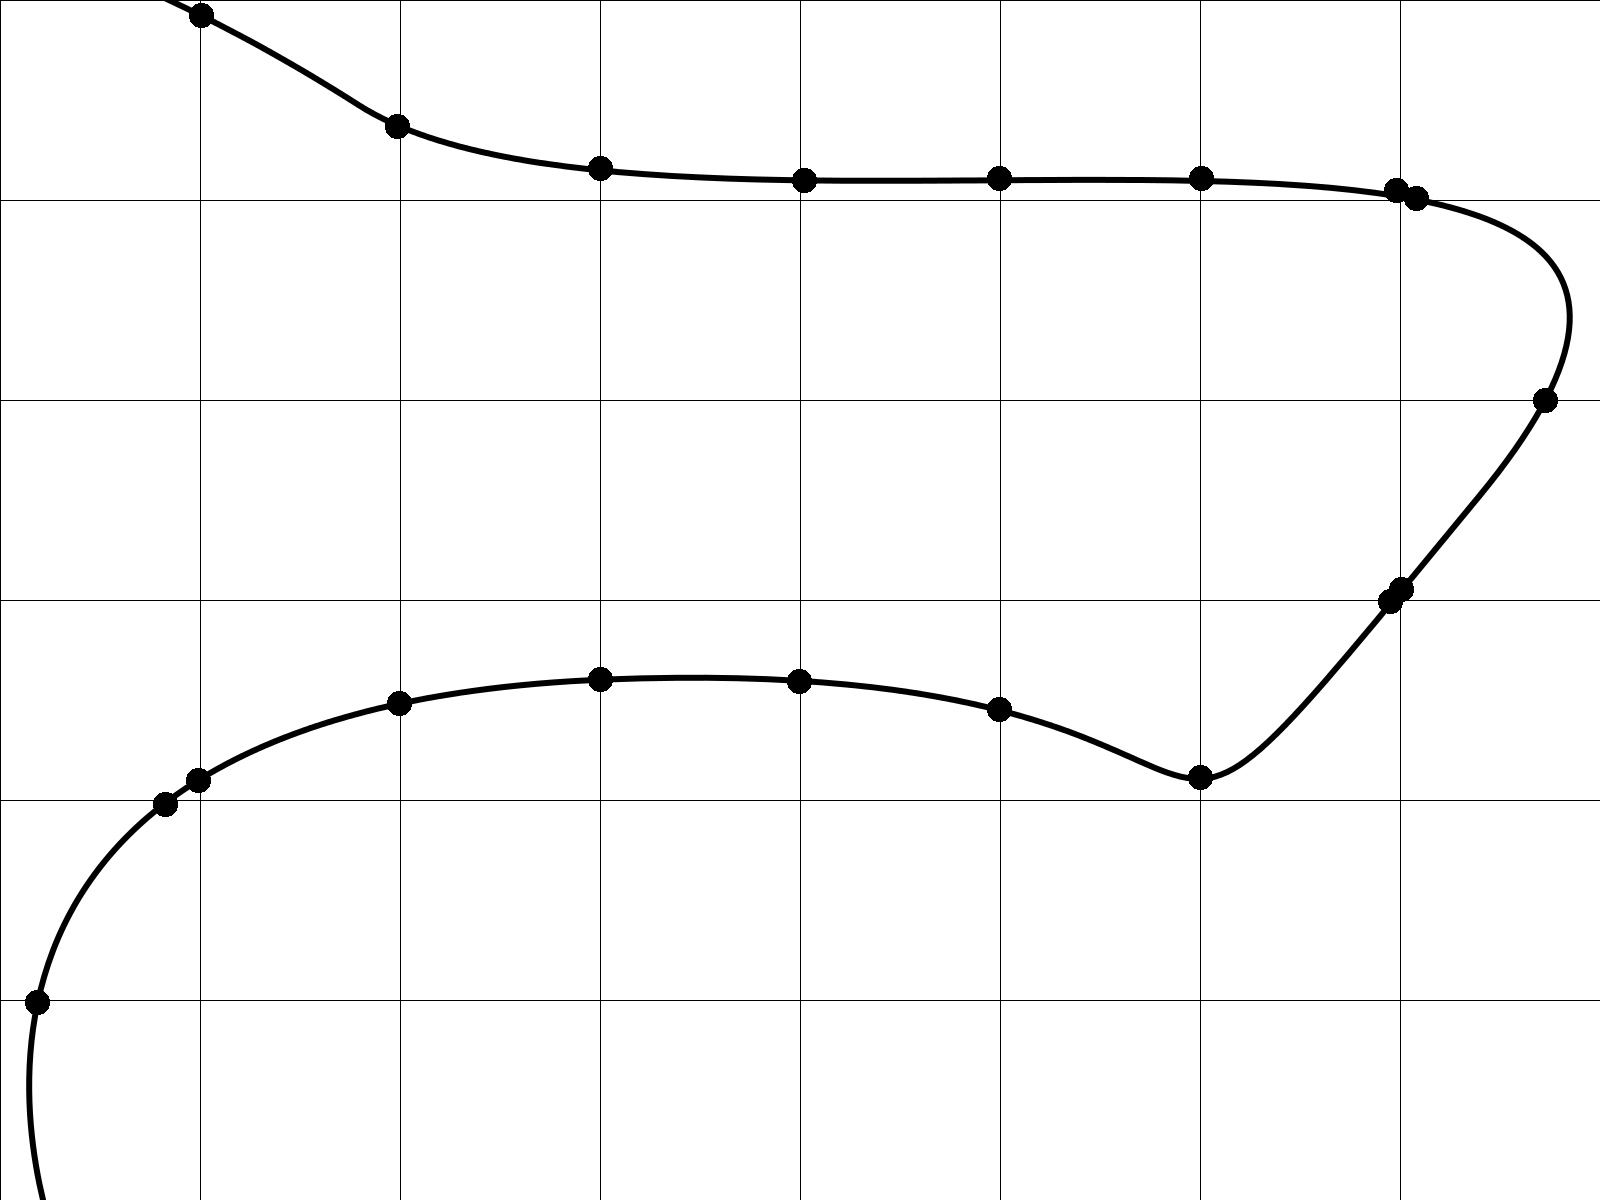
\includegraphics[width=0.9\textwidth]{diagrams/2DGrid}
    \caption{This diagram shows the effect of an extra dimension on the number of grid crossings.
    In a 2D problem, corrections would need to be made at every point where there is a dot.
    If the interface were moving, this would potentially have to be redone at every timestep, in addition to doing corrections in the time dimension.}
    \label{2DGrid}
\end{figure}

The addition of extra interface-grid crossings requires extra corrections.
Although these corrections are not complex to derive based on any of the three above methods, their implementation is where difficulties arise.
Properly accounting for every possible combination of grid crossings is a difficult task to accomplish programattically, and this is one disadvantage of the IIM not shared by smoothing methods.
